%\setchapterimage{Fond_SLCI.png}
\setchapterpreamble[u]{\margintoc}

\chapter{Introduction à quelques méthodes numériques}

\marginnote[5cm]{
\UPSTIcompetence[2]{C3-02}
%\UPSTIcompetence[2]{C2-04}
}

%

\begin{obj}[ -- C3-02 : Résoudre numériquement une équation ou un système d'équations ]
\begin{itemize}
\item Réécriture des équations d'un problème;
\item résolution de problèmes du type f(x) = 0 (méthodes de dichotomie et de Newton);
\item résolution d'un système linéaire du type $A\cdot X = B$;
\item résolution d'équations différentielles (schéma d'Euler explicite);
\item intégration et dérivation numérique (schémas arrière et avant).
\end{itemize}
\end{obj}



\section{Equations stationnaires -- Résolution de $f(x)=0$}

\subsection{Principe de la méthode de dichotomie}

\begin{marginfigure}
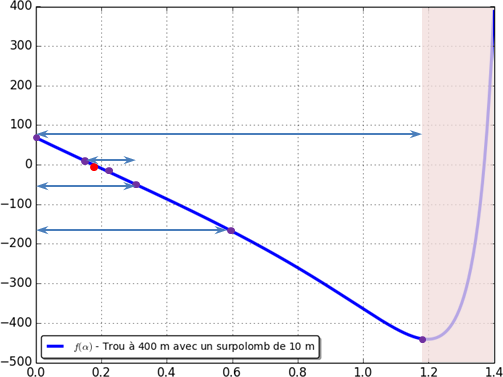
\includegraphics[width=\linewidth]{InterpretationG}
\end{marginfigure}

\begin{theoreme}[Théorème des valeurs intermédiaires]

Soit $f$ une fonction définie et continue sur l'intervalle $[a,b]$ à valeur dans $\mathbb{R}$. Pour tout $u\in[f(a),f(b)]$, il existe au moins un réel $c\in [a,b]$  tel que $f(c)=u$.

 En particulier (Théorème de Bolzano), si $f(a)$ et $f(b)$ sont de signes différents, il existe au moins un réel $c$ tel que $f(c)=0$. 
\end{theoreme}


Ainsi, pour une fonction donnée définie sur un intervalle donné, le but de l'algorithme de dichotomie va être de découper en 2 l'intervalle [a,b] en deux, afin d'y trouver la solution. Par divisions successives de l'intervalle, on convergera vers la solution.


\begin{remarque}
\textbf{Tester le signe de $f(a)$ et $f(b)$.}

Il existe plusieurs méthodes pour tester si $f(a)$ et $f(b)$ sont de signes différents. Si on ne se préoccupe pas de savoir la relation d'ordre entre $f(a)$ et $f(b)$, un test efficace consiste en un test du signe de $f(a)\cdot f(b)$. 
\end{remarque}




\subsection{Principe de la méthode de Newton}
\begin{defi}[Développement de Taylor à l'ordre 1]

Soit $f$ une fonction $C^1$ sur un intervalle $I$ et $a\in I$. Le développement de Taylor à l'ordre 1 de $f$ est donné par 
$$
f(x)=f(a)+ f'(a)\cdot(x-a)+\mathit{o}(x-a)
$$
\end{defi}



Géométriquement, lorsqu'on néglige le reste, le développement de Taylor donne l'équation de la tangente en $a$. Notons $\Delta(x)$ cette équation.

L'abscisse $c$ de l'intersection de la tangente avec l'axe des abscisses est donnée par la résolution de 
$$
\Delta(c)=0 
\Longleftrightarrow f(a)+ f'(a)\cdot(c-a) = 0
\Longleftrightarrow c = a-\dfrac{f(a)}{f'(a)}
$$


\begin{marginfigure}
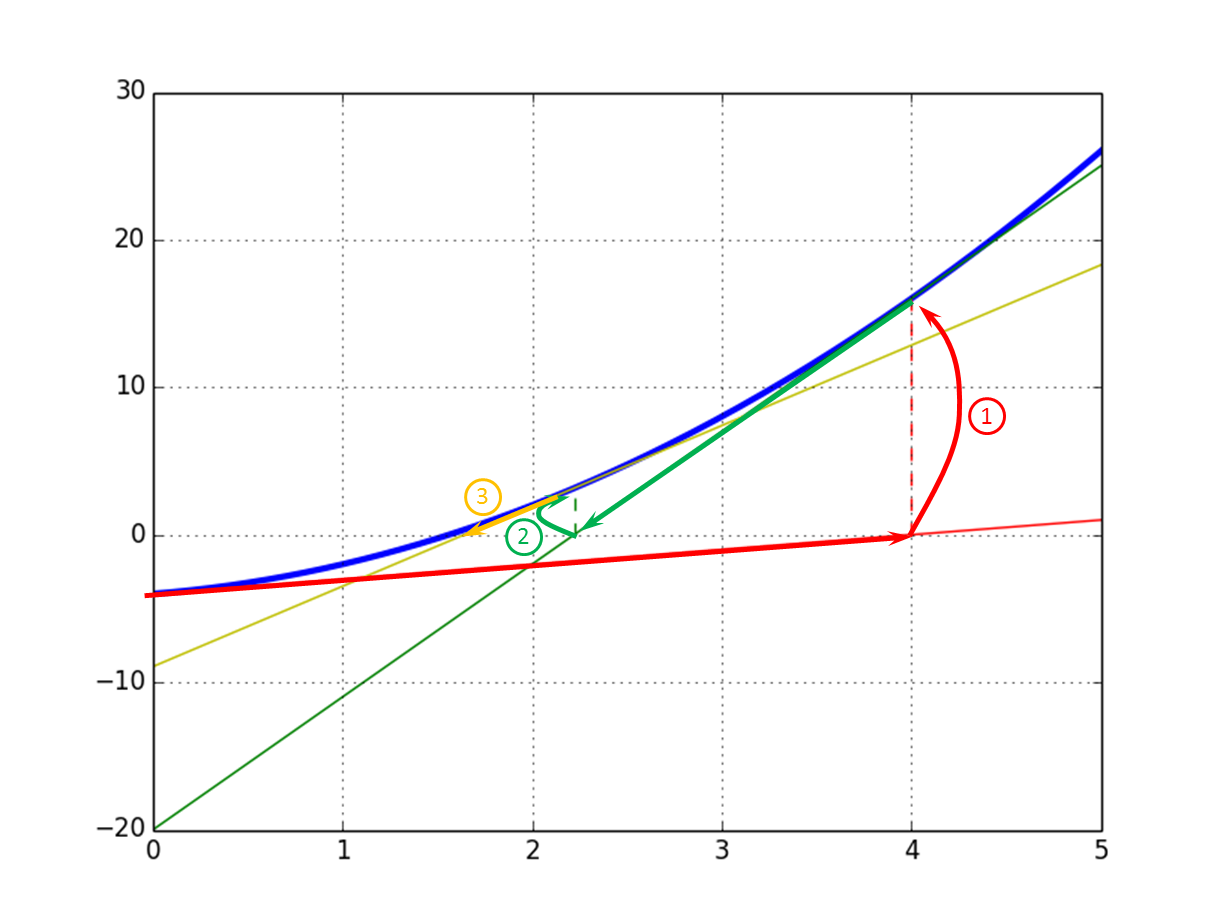
\includegraphics[width=\linewidth]{interpretation_newton}
\end{marginfigure}


\subsection*{Évaluation de la dérivée numérique}

\begin{resultat}
En première approximation, il est possible d'approximer la dérivée en approximant la tangente à la courbe par une droite passant par deux points successifs. Dans ces conditions, pour une valeur de $h$ suffisamment faible, on a : 
$$
f'(x_0)\simeq \dfrac{f(x_0+h)-f(x_0)}{h}.
$$
\end{resultat}


%
%\begin{resultat}
%\textbf{Théorème de Taylor-Young}
%Si $f$ est deux fois dérivable en $x_0$ et $f''(x_0)\neq 0$, 
%$$
% \dfrac{f(x_0+\varepsilon)-f(x_0)}{\varepsilon} - f'(x_0) \sim \dfrac{f''(x_0)}{2}h
%$$
%\end{resultat}%

\subsubsection{Méthodes à un pas}


\begin{resultat}
\textbf{Différence avant -- Schéma d'Euler explicite}

Dans ce cas, l'estimation de la dérivée au point $P_i$ s'appuie sur le point $P_{i+1}$ :
$$
f'(x_i)\simeq\dfrac{f(x_{i+1})-f(x_i)}{x_{i+1}-x_i}
$$
\end{resultat}


\begin{marginfigure}
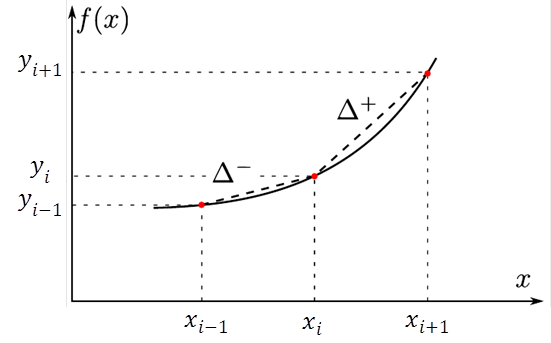
\includegraphics[width=\textwidth]{derivation_1pas}
\end{marginfigure}

\begin{resultat}[Différence arrière -- Schéma d'Euler implicite]

Dans ce cas, l'estimation de la dérivée au point $P_i$ s'appuie sur le point $P_{i-1}$ :
$$
f'(x_i)\simeq\dfrac{f(x_{i})-f(x_{i-1})}{x_{i}-x_{i-1}}
$$
\end{resultat}


\subsubsection{Méthode à deux pas}

\begin{marginfigure}
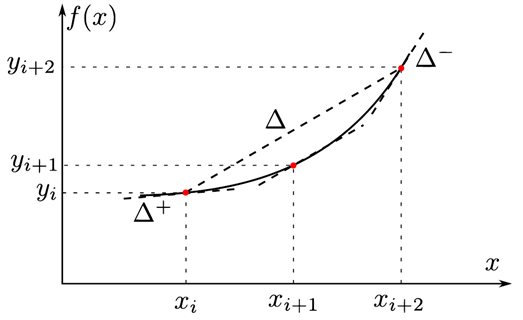
\includegraphics[width=\textwidth]{derivation_2pas}
\end{marginfigure}

\begin{resultat}
On peut aussi utiliser les points $P_{i-1}$ et $P_{i+1}$ pour estimer la dérivée en $P_i$ :
$$
f'(x_i)\simeq\dfrac{f(x_{i+1})-f(x_{i-1})}{x_{i+1}-x_{i-1}}
$$
\end{resultat}

\begin{remarques}
\begin{itemize}
\item Lorsqu'il s'agit de dériver une fonction temporelle « en temps réel », le point suivant n’est pas encore connu donc seule la différence arrière peut être calculée.
\item Le calcul de la dérivée conduit à un tableau de valeurs de dimension $n-1$.
\end{itemize}
\end{remarques}



\subsection{Bibliothèque Python}
Il est possible de résoudre l'équation $f(x)=0$ en utilisant les modules de la bibliothèque \texttt{scipy} :
%\begin{py}

Résolution de $\sin(x)=0$ avec 0,5 comme valeur d'initialisation.
\begin{lstlisting}
def f(x):
    return sin(x)
   
sol = newton(f,0.5)
print(sol)
print(f(sol))
\end{lstlisting}

Résolution du système : 
$$
\left\{\begin{array}{l} 
x+10y-3z-5 = 0 \\ 
2x-y+2z-2 = 0\\
 -x+y+z+3 = 0\end{array}\right.
 $$


\begin{lstlisting}
from scipy.optimize import fsolve
# définition du système
def syst(var): 
    # définition des variables
    x, y, z = var[0], var[1], var[2] 
    eq1 = x +10*y-3*z-5
    eq2 = 2*x-y+2*z-2
    eq3 = -x+y+z+3
    res = [eq1, eq2, eq3]
    return res
    # Initialisation de la recherche 
    # des solutions numériques
x0, y0, z0 = 0, 0, 0 
sol_ini = [x0, y0, z0]
sol = fsolve(syst, sol_ini)
sol = newton(f,0.5)
print(sol)
\end{lstlisting}


%\end{py}


\section{Intégration numérique}

\begin{hypo}  $f:[a,b]\rightarrow \mathbb{R}$ est une fonction continue sur $[a,b]$. On note $I = \int\limits_a^{b} f(x) \mathrm{d}x $.
\end{hypo}

\subsection{Principe des méthodes des rectangles}
%\subsection{Principe}
\begin{defi}[Méthode des rectangles]
Dans cette méthode, la fonction à intégrer est interpolée par un polynôme de degré 0, à savoir une fonction constante. Géométriquement, l'aire sous la courbe est alors approximée par un rectangle. Plusieurs choix sont possibles.

\begin{itemize}
\item Rectangles à gauche : $ I = \int\limits_a^{b} f(x) \mathrm{d}x \simeq \left(b-a\right) f(a). $
\item Point milieu : $ I = \int\limits_a^{b} f(x) \mathrm{d}x \simeq \left(b-a\right) f\left(\dfrac{a+b}{2}\right). $
\item Rectangles à droite :  $ I = \int\limits_a^{b} f(x) \mathrm{d}x \simeq \left(b-a\right) f(b). $
\end{itemize}

\end{defi}

\subsection{Interprétation graphique}

\begin{minipage}[c]{.24\linewidth}
\begin{center}
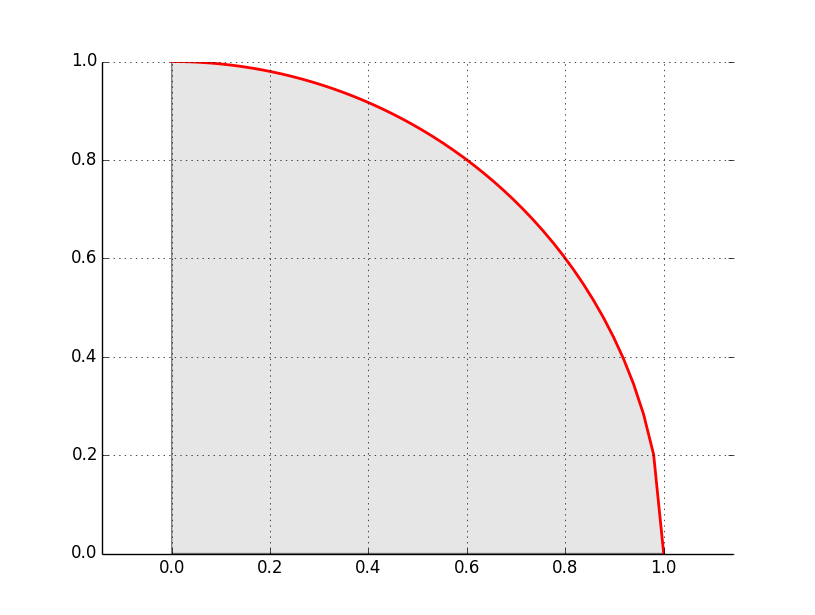
\includegraphics[width=.99\textwidth]{pi_courbe}

\textit{Calcul intégral}
\end{center}
\end{minipage}\hfill
\begin{minipage}[c]{.24\linewidth}
\begin{center}
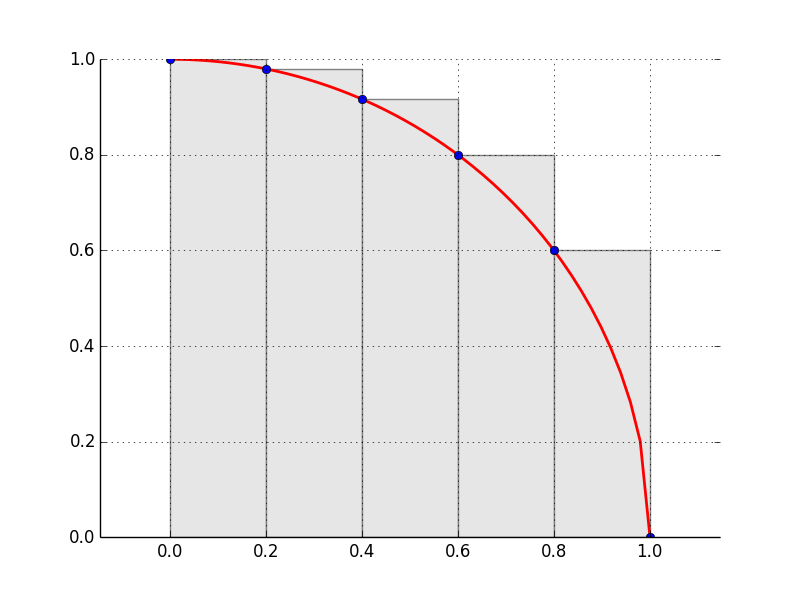
\includegraphics[width=.99\textwidth]{pi_rect_g}

\textit{Rectangles à gauche}
\end{center}
\end{minipage}\hfill
\begin{minipage}[c]{.24\linewidth}
\begin{center}
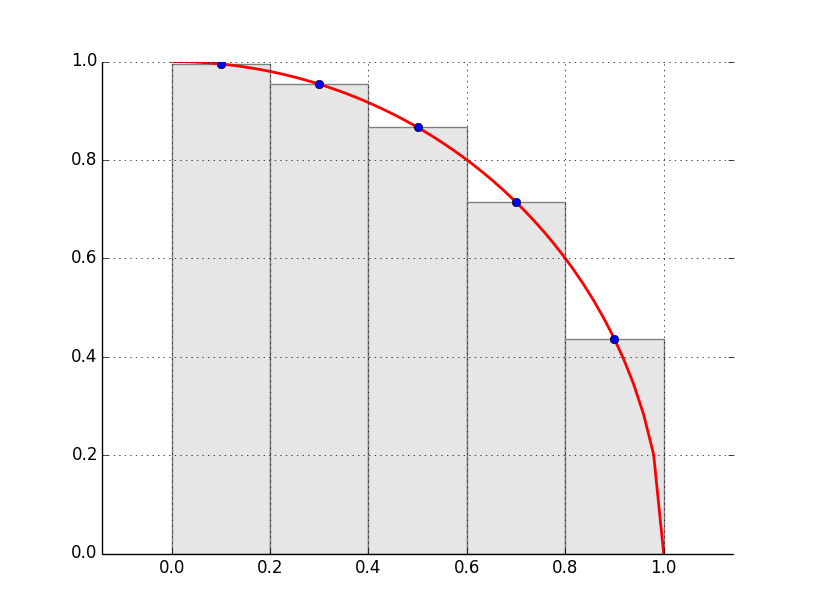
\includegraphics[width=.99\textwidth]{pi_rect_m}

\textit{Point milieu}
\end{center}
\end{minipage}\hfill
\begin{minipage}[c]{.24\linewidth}
\begin{center}
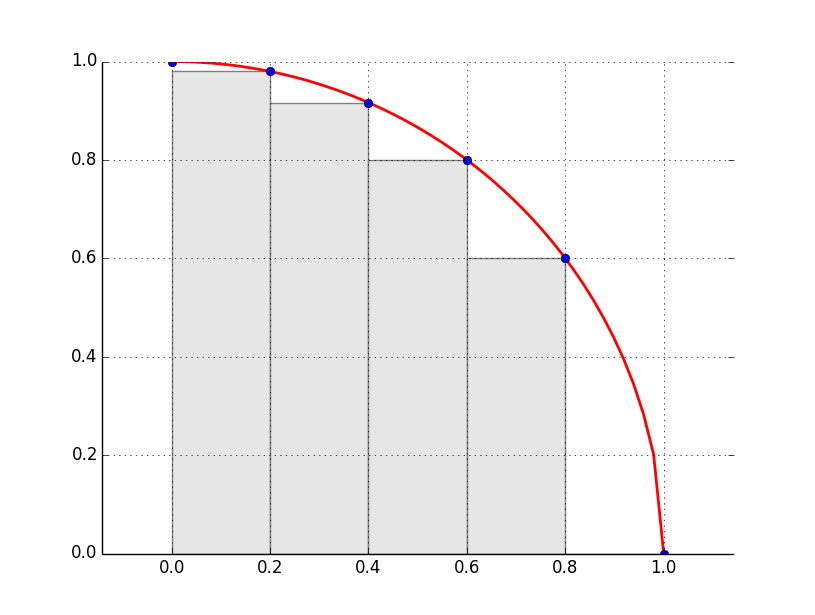
\includegraphics[width=.99\textwidth]{pi_rect_d}

\textit{Rectangles à droite}
\end{center}
\end{minipage}


\subsection{Principe des méthodes des trapèzes}


\begin{marginfigure}
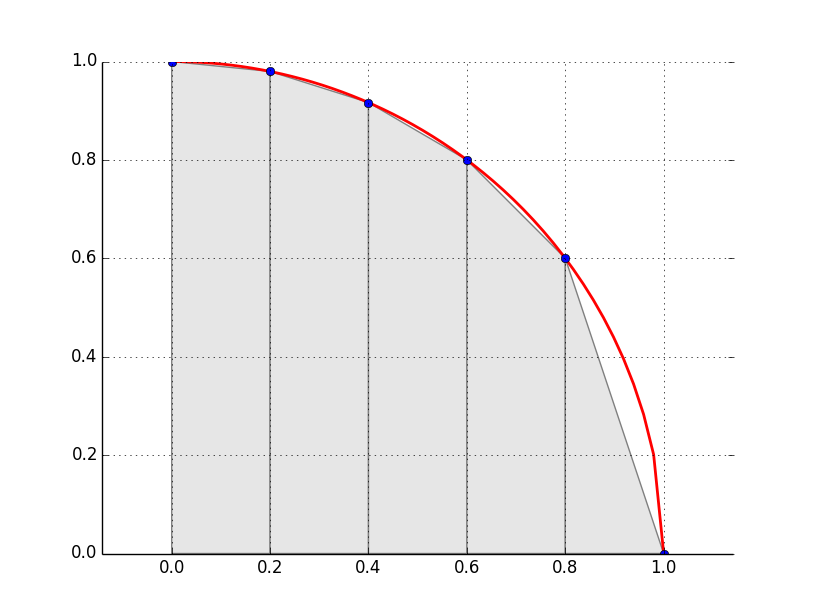
\includegraphics[width=.99\textwidth]{pi_trap}
\end{marginfigure}

\begin{defi}{Méthode des trapèzes}
Dans cette méthode, la fonction à intégrer est interpolée par un polynôme de degré 1, à savoir une fonction affine. Géométriquement, l'aire sous la courbe est alors approximée par un trapèze :

$$
I = \int\limits_a^{b} f(x) \mathrm{d}x \simeq \left(b-a\right) \dfrac{f(a)+f(b)}{2} 
$$
\end{defi}




\subsection*{Notion d'erreur d'intégration}
\begin{resultat}
Dans chaque cas,  on intègre $f$ sur $n$ subdivisions régulières de $I$. 

\textbf{Erreur sur la méthode des rectangles à gauche et à droite}

Soit $f$ fonction dérivable sur $I=[a,b]$ et dont $f'$ est continue sur $I$. Soit $M_1$ un majorant de $f'$ sur $I$. L'erreur $\varepsilon$ commise lors de l'intégration par la méthode des rectangles à droite ou à gauche
 est telle que $ \varepsilon \leq \dfrac{M_1}{2n}$.

\textbf{Erreur sur la méthode des rectangles -- point milieu}

Si de plus $f$ est deux fois dérivables sur $I=[a,b]$ et $f''$ est continue sur $I$, on note $M_2$ un majorant de $f''$ sur $I$.L'erreur $\varepsilon$ commise lors de l'intégration par la méthode des rectangles -- point milieu est telle que $ \varepsilon \leq \dfrac{M_2}{12n^2}$.

\textbf{Erreur sur la méthode des trapèzes}

L'erreur commise $\varepsilon$ est telle qu'il existe un entier $M$ tel que $ \varepsilon \leq \dfrac{M}{12n^2}$.

\end{resultat}

\subsection*{Bibliothèque Python}
Il est possible d'intégrer une fonction en utilisant les modules de la bibliothèque \texttt{scipy} :
\begin{lstlisting}
from scipy.integrate import quad
from math import sin
# Définition des bornes de gauche et de droite
g,d = -1,1 
def f(x):
    return sin(x)
   
I,erreur = quad(f,g,d)
print(I,erreur)
\end{lstlisting}


\section{Résolution d'équations différentielles}


\subsection{Problème de Cauchy}

Le problème consiste à trouver les fonctions $y$ de $[0,T]\rightarrow \mathbb{R}^n$ telles que
$$
\left\{
\begin{array}{l}
\dfrac{\text{d} y(t)}{\text{d} t}=f(t,y(t)) \\
y(t_0)=y_0 \quad \text{avec } t_0\in [0,T] \text{ et } y_0\in \mathbb{R}^n \text{ donnés}
\end{array}
\quad \text{avec } t_0\in [0,T] \text{ et } y_0\in \mathbb{R}^n \text{ donnés.}
\right.
 $$ 

L'existence et l'unicité de la solution peut se démontrer en utilisant le théorème de Cauchy-Lipschitz.


\begin{defi}[Fonction lipschitzienne]

$f$ est lipschitzienne en $y$ s'il existe un réel $k>0$ tel que $\forall y(t)\in\mathbb{R}^n$, $\forall z(t)\in\mathbb{R}^n$, $\forall t\in[0,T]$, alors 
$$
||f(t,y(t))-f(t,z(t))||\leq k||y(t)-z(t)||
$$

\end{defi}

\begin{theoreme}[Théorème de Cauchy -- Lipschitz]

Soit $f$ une fonction de $[0,T] \times \mathbb{R}^n \rightarrow \mathbb{R}^n$ continue et lipschitzienne en $y$. 

Alors, $\forall t_0 \in [0,T]$ et $\forall y_0 \in \mathbb{R}^n$, le problème de Cauchy admet une unique solution définie sur $[0,T]$.

\end{theoreme}

\subsection{Méthode d'Euler}
Pour un temps de simulation compris entre $t_0$ et $t_1$, si on choisi un nombre $n$ d'échantillons, alors le pas d'intégration est défini par  $h=\dfrac{t_1-t_0}{n}$. (On a donc $t_i = t_0+h\cdot i$ avec $i\in[0,n]$.)

\begin{resultat}
En intégrant l'équation du problème de Cauchy sur un intervalle $[t_i, t_{i+1}]$, on a : 
$$
\int\limits_{y_i}^{y_{i+1}} \text{d}y = \int\limits_{t_i}^{t_{i+1}} f(t,y(t)) \text{d}t 
$$

$$
\Leftrightarrow 
y_{i+1} - y_i = \int\limits_{t_i}^{t_{i+1}} f(t,y(t)) \text{d}t  \text{ et donc : }  y_{i+1}= y_i + \int\limits_{t_i}^{t_{i+1}} f(t,y(t)) \text{d}t 
$$

 En utilisant la méthode des rectangles à gauche, $\int\limits_{t_i}^{t_{i+1}} f(t,y(t)) \text{d}t  \simeq h \cdot f(t_i,y(t_i)) $.

\end{resultat}


\subsection{Méthode d'Euler explicite}

À l'instant $i$, $\dfrac{\text{d}y(t)}{\text{d}t}$ peut être approximé par 
$\dfrac{\text{d}y(t_i)}{\text{d}t} \simeq \dfrac{y_{i+1}-y_i}{h}$.
Ainsi, $y_{i+1} = y_i +h  f(t_i,y_i)$.

\subsection*{Méthode d'Euler implicite}
À l'instant $i$, $\dfrac{\text{d}y(t)}{\text{d}t}$ peut être approximé par 
$\dfrac{\text{d}y(t_{i})}{\text{d}t} \simeq \dfrac{y_{i}-y_{i-1}}{h}$.
Ainsi, $y_{i} = y_{i-1} +h  f(t_{i-1},y_{i})$ ou encore $y_{i+1} = y_{i} +h  f(t_{i},y_{i+1})$.
\subsection*{Bibliothèque Python}

Voir exemples : \url{http://python.physique.free.fr/outils_math.html}.


\subsection{Exemples -- Reformulation d'équations différentielles en vue de leur résolution numérique.}
\subsubsection{Équation différentielle du premier ordre à coefficients constants}
On a $\omega(t) + \tau \dfrac{\text{d} \omega(t)}{\text{d}t} = \omega_c $.

En utilisant la formulation du problème de Cauchy, on a $f(t,y(t)) = \deriv{\omega(t)}{} = \dfrac{1}{\tau}\left(\omega_c - \omega(t)\right)$.




Pour la méthode d'Euler explcite, on a donc, $\omega[k+1]=\omega[k]+\dfrac{h}{\tau}\left(\omega_c - \omega[k]\right)$.
\marginnote[-4cm]{On retrouve la même chose en discrétisant l'équation différentielle : pour un schéma d'Euler explicite, on a $\dfrac{\text{d} \omega(t)}{\text{d}t}\simeq \dfrac{\omega_{k+1}-\omega_k}{h} \Rightarrow  \omega_k + \tau  \dfrac{\omega_{k+1}-\omega_k}{h} = \omega_c  \Leftrightarrow \omega_{k+1} =\dfrac{h}{\tau} \left(\omega_c - \omega_k\right)+\omega_k$.}



Pour la méthode d'Euler implicite, on a $\omega[k+1]=\omega[k]+\dfrac{h}{\tau}\left(\omega_c - \omega[k+1]\right)$ 
$\Leftrightarrow \omega[k+1] \left(1+\dfrac{h}{\tau}\right) =\omega[k] + \dfrac{h}{\tau}\omega_c$ 
$\Leftrightarrow \omega[k+1] \left(1+\dfrac{h}{\tau}\right) =\dfrac{\tau}{1+h}\left(\omega[k] + \dfrac{h}{\tau}\omega_c\right)$.
\marginnote[-3cm]{Avec le schéma d'Euler implicite: on a $\dfrac{\text{d} \omega(t)}{\text{d}t}\simeq \dfrac{\omega_{k}-\omega_{k-1}}{h} \Rightarrow  \omega_k + \tau  \dfrac{\omega_{k}-\omega_{k-1}}{h} = \omega_c  \Leftrightarrow   \omega_k = \dfrac{h\omega_c + \tau\omega_{k-1}}{h+\tau} $.}


\subsubsection{Équation différentielle du premier ordre à coefficients non constants}

\begin{itemize}[label=\ding{112},font=\color{red}] 
\item   $\omega(t) f(t) + \tau \dfrac{\text{d} \omega(t)}{\text{d}t} g(t)  = \omega_c h(t)$ :
\begin{itemize}
\item Euler explicite : $\dfrac{\text{d} \omega(t)}{\text{d}t}\simeq \dfrac{\omega_{k+1}-\omega_k}{h} \Rightarrow  \omega_k f_k+ \tau  \dfrac{\omega_{k+1}-\omega_k}{h} g_k= \omega_c h_k  \Leftrightarrow \omega_{k+1} =\dfrac{h}{\tau g_k} \left(\omega_c h_k - \omega_k f_k \right)+\omega_k$;
\item Euler implicite : $\dfrac{\text{d} \omega(t)}{\text{d}t}\simeq \dfrac{\omega_{k}-\omega_{k-1}}{h} \Rightarrow  \omega_k f_k+ \tau \dfrac{\omega_{k}-\omega_{k-1}}{h} g_k= \omega_c h_k  \Leftrightarrow \omega_k =  \dfrac{h\omega_c h_k +\tau g_k\omega_{k-1}}{f_k h+   \tau g_k}  $.
\end{itemize}
\end{itemize}


\subsubsection{Équation différentielle du premier ordre}

\begin{itemize}[label=\ding{112},font=\color{red}] 
\item  $\sin \left(\omega(t)\right) + \dfrac{\text{d}\omega(t)}{\text{d}t}=K$ :
\begin{itemize}
\item Euler explicite : $\dfrac{\text{d} \omega(t)}{\text{d}t}\simeq \dfrac{\omega_{k+1}-\omega_k}{h} \Rightarrow  \sin \omega_k +  \dfrac{\omega_{k+1}-\omega_k}{h}=K \Leftrightarrow  \omega_{k+1}=h\left( K - \sin \omega_k\right)+\omega_k$;
\item Euler implicite : $\dfrac{\text{d} \omega(t)}{\text{d}t}\simeq \dfrac{\omega_{k}-\omega_{k-1}}{h} \Rightarrow \sin \omega_k +  \dfrac{\omega_{k}-\omega_{k-1}}{h}=K \Leftrightarrow h\sin \omega_k +  \omega_{k}-\omega_{k-1}=hK$. Dans ce cas, il faut utiliser la méthode de Newton ou de dichotomie pour déterminer $\omega_k$.
\end{itemize}

\end{itemize}


\subsubsection{Équation différentielle du second ordre}

 Soit l'équation $\ddot{s}(t) + \dfrac{2\xi}{\omega_0} \dot{s}(t) + \omega_0^2 s(t) = Ke(t)$ avec $s(0)=0$ et $\dot{s}(t)=0$
En utilisant le problème de Cauchy, on pose : 
$Y(t)=
\left\{
\begin{array}{l}
y_1(t) = s(t) \\
y_2(t) = \dot{s}(t) \\
\end{array}
\right.$
$\Rightarrow 
\left\{
\begin{array}{l}
\dot{y_1}(t) = \dot{s}(t) = y_2(t) \\
\dot{y_2}(t) = \ddot{s}(t) \\
\end{array}
\right.
\Rightarrow 
\left\{
\begin{array}{l}
\dot{y_1}(t) = y_2(t) \\
\dot{y_2}(t) =  Ke(t) - \dfrac{2\xi}{\omega_0} y_2(t)- \omega_0^2 y_1(t) \\
\end{array}
\right.
$

En utilisant le schéma d'euler explicte on a donc $Y[k+1] = Y[k]+h
\left[
\begin{array}{l}
y_2[k] \\
Ke[k] - \dfrac{2\xi}{\omega_0} y_2[k]- \omega_0^2 y_1[k] \\
\end{array}
\right]$

et donc 
$
\left[
\begin{array}{l}
y_1[k+1] \\
y_2[k+1] \\
\end{array}
\right]
=\left[
\begin{array}{l}
y_1[k] \\
y_2[k] \\
\end{array}
\right]
+
h
\left[
\begin{array}{l}
y_2[k] \\
Ke[k] - \dfrac{2\xi}{\omega_0} y_2[k]- \omega_0^2 y_1[k] \\
\end{array}
\right]
$
$=
\left[
\begin{array}{l}
y_1[k]+hy_2[k] \\
y_2[k]+h\left(Ke[k] - \dfrac{2\xi}{\omega_0} y_2[k]- \omega_0^2 y_1[k] \right)\\
\end{array}
\right]
$
\footnotesize{

Schéma d'Euler explicite :   $\dfrac{\text{d} y(t)}{\text{d}t}\simeq \dfrac{y_{k+1}-y_k}{h}$. On a donc :
$$
\left\{
\begin{array}{l}
\dfrac{y_{1,k+1}-y_{1,k}}{h} = y_{2,k} \\
\dfrac{y_{2,k+1}-y_{2,k}}{h} + \dfrac{2\xi}{\omega_0} y_{2,k}+ \omega_0^2 y_{1,k} = Ke_k \\
\end{array}
\right.
$$ 

$$\Leftrightarrow 
\left\{
\begin{array}{l}
y_{1,k+1} = h y_{2,k} +y_{1,k} \\
y_{2,k+1}  = hKe_k - \dfrac{2\xi h}{\omega_0} y_{2,k}- h\omega_0^2 y_{1,k} + y_{2,k}\\
\end{array}
\right.
$$ 


Schéma d'Euler implicite: $\dfrac{\text{d} y(t)}{\text{d}t}\simeq \dfrac{y_{k}-y_{k-1}}{h}$. On a donc :
$$
\left\{
\begin{array}{l}
\dfrac{y_{1,k}-y_{1,k-1}}{h} = y_{2,k} \\
\dfrac{y_{2,k}-y_{2,k-1}}{h} + \dfrac{2\xi}{\omega_0} y_{2,k}+ \omega_0^2 y_{1,k} = Ke_k \\
\end{array}
\right.$$
$$
\Leftrightarrow 
\left\{
\begin{array}{l}
y_{1,k} = hy_{2,k}+y_{1,k-1} \\
y_{2,k} =\dfrac{h Ke_k+y_{2,k-1} - h\omega_0^2 y_{1,k-1}}{1+  h \dfrac{2\xi}{\omega_0} +  \omega_0^2 h^2 } \\
\end{array}
\right.$$

\normalsize


\subsubsection{Suite ...}
\begin{itemize}[label=\ding{112},font=\color{red}] 
\item Équation différentielle du second ordre : $\ddot{\theta}(t) + k \sin \theta(t) = 0$.
On pose : 
$$
\left\{
\begin{array}{l}
y_0(t) = \theta(t) \\
y_1(t) = \dot{\theta}(t) \\
\end{array}
\right. 
\Rightarrow 
\left\{
\begin{array}{l}
\dot{y_0}(t) = \dot{\theta}(t) = y_1(t) \\
\dot{y_1}(t) = \ddot{\theta}(t) \\
\end{array}
\right.
\Rightarrow 
\left\{
\begin{array}{l}
\dot{y_0}(t) = y_1(t) \\
\dot{y_1}(t) + k \sin y_0 (t) = 0 \\
\end{array}
\right.
$$



\begin{center}
\begin{tabular}{p{.47\linewidth}|p{.47\linewidth}}
Schéma d'Euler explicite :   

$
\left\{
\begin{array}{l}
\dfrac{y_{0,k+1}-y_{0,k}}{h} = y_{1,k} \\
\dfrac{y_{1,k+1}-y_{1,k}}{h} + k \sin y_{0,k} = 0 \\
\end{array}
\right.$

$\Leftrightarrow 
\left\{
\begin{array}{l}
y_{0,k+1} = h y_{1,k} +y_{0,k} \\
y_{1,k+1} = y_{1,k} - kh \sin y_{0,k} \\
\end{array}
\right.$
&
Schéma d'Euler implicite : 

$
\left\{
\begin{array}{l}
\dfrac{y_{0,k}-y_{0,k-1}}{h} = y_{1,k} \\
\dfrac{y_{1,k}-y_{1,k-1}}{h} + k \sin y_{0,k} = 0 \\
\end{array}
\right.$

$\Leftrightarrow 
\left\{
\begin{array}{l}
y_{0,k} = h y_{1,k}+y_{0,k-1} \\
y_{1,k} = y_{1,k-1} - kh \sin y_{0,k} \\
\end{array}
\right.$.
\end{tabular}
\end{center}


%\item Équation différentielle du second ordre : $(k_1+k_2  \sin^2 \theta(t) ) \ddot{\theta}(t)+ (k_3 \dot{\theta}(t)^2+k_4) \sin 2\theta(t) +C(t)=0$.

\end{itemize}
\subsection{Bibliothèque Python}

\section{Résolution de systèmes linéaires}
\subsection{Utilisation du pivot de Gauss}

Le pivot de Gauss est une méthode permettant de résoudre les systèmes linéaires. Sur l'idée du pivot de Gauss, il est alors possible de calculer l'inverse d'une matrice (lorsqu'elle est inversible), de calculer le déterminant d'une matrice $A\in\mathcal{M}_n(\mathbb{R})$ ou de calculer le rang de 
$A\in\mathcal{M}_{n,p}(\mathbb{R})$.

Outre la compréhension et la mise en \oe{}uvre de l'algorithme, deux problèmes numérique peuvent se poser : 
\begin{itemize}
\item les erreurs d'arrondis peuvent provoquer des erreurs importantes selon la méthode choisie;
\item des comparaisons d'un réel à zéro peuvent aussi engendrer des erreurs numériques.
\end{itemize}

\begin{remarque}
Les résultats du cours sont écrits avec des coefficients réels mais restent vrais avec des coefficients complexes. 
\end{remarque}

\subsubsection{Définitions}
\begin{defi}[Système linéaire]
On dit d'un système qu'il est linéaire s'il est de la forme :
$$
\left\{
\begin{array}{l}
a_{11}x_1 + a_{12}x_2 + ... + a_{1p}x_p = b_1 \\
... \\ 
a_{n1}x_1 + a_{n2}x_2 + ... + a_{np}x_p = b_n \\
\end{array}
\right.
$$

On note $n,p\in \mathbb{N}^*$ ($n$ équations et $p$ inconnues), $\forall i\in \{1,...,n\}$, $\forall j\in \{1,...,p\}$, $a_{ij} \in \mathbb{R}$. $i$ désigne l'indice de la ligne et $j$ l'indice de la colonne. 

$b_1, ..., b_n \in \mathbb{R}$ est appelé second membre. 
\end{defi}

\begin{defi}[Système homogène]
On dit que le système est homogène su $b_1=b_2=...=b_n=0$.
\end{defi}


\begin{exemple}
Exemple de système linéaire $(S)$ et son système homogène associé $(S_0)$ :
$$
(S) \left\{
\begin{array}{l}
x+y-2z + 4t = 5 \\
2x+2y-3z+t=3 \\
3x+3y-4z-2t=1
\end{array}
\right.
\quad
(S_0) \left\{
\begin{array}{l}
x+y-2z + 4t = 0 \\
2x+2y-3z+t=0 \\
3x+3y-4z-2t=0
\end{array}
\right.
$$

Exemple de système non linéaire :
$$
\left\{
\begin{array}{l}
x+\mathbf{\cos y} + \mathbf{xy} =2 \\
x-\mathbf{y^2} = 4
\end{array}
\right.$$

\end{exemple}

\begin{defi}[Système linéaire]
Une solution d'un système linéaire est un p-uplet de réels, c'est-à-dire un élément de $(x_1,...,x_p)$ qui vérifie les $n$ équations. 
\end{defi}


\begin{defi}[Système compatible]
Si un système a au moins une solution, il est dit compatible (incompatible sinon).
\end{defi}


\subsubsection{Opérations élémentaires}
\begin{defi}
Les opérations élémentaires sont les suivantes :
\begin{itemize}
\item opération de transvection (\textit{Gaussian Elimination}): 
\begin{itemize}
\item $(L_i)\leftarrow (L_i)+\lambda (L_j)$ où $i,j\in \{1,...,n\}$, $i\neq j$, $\lambda \in \mathbb{R}$;
\item $(L_i)\leftarrow \alpha (L_i)$ où $i\in \{1,...,n\}$, $\alpha \in \mathbb{R}^*$;
\end{itemize}
\item opération d'échange de lignes : 
\begin{itemize}
\item $(L_i)\leftrightarrow  (L_j)$ où $i,j\in \{1,...,n\}$. 
\end{itemize}
\end{itemize}
\end{defi}

\begin{remarque}
Pour éviter les fractions on peut également utiliser $(L_i)\leftarrow \alpha (L_i) + \lambda L_j$ où $i,j\in \{1,...,n\}$, $\alpha \neq 0$, $\lambda \in \mathbb{R}$ qui est une combinaison des deux premiers items.
\end{remarque}

\begin{proposition}
L'utilisation des opérations élémentaires sur un système ne change pas l'ensemble de ses solutions. Autrement dit, elles donnent des systèmes équivalents au premier.
\end{proposition}

\subsubsection{Notation matricielle}
\begin{remarque}
Les opérations élémentaires sur les lignes du système n'opèrent que sur les coefficients. 
\end{remarque}

\begin{defi}{}
Au système défini précédemment, on associe la matrice de ses coefficients :
$$
\begin{pmatrix}
a_{11} & a_{12} & \ldots & a_{1(p-1)} & a_{1p} \\
 & & a_{ij} & & \\
a_{n1} & a_{n2} & \ldots & a_{n(p-1)} & a_{np} \\
\end{pmatrix} \in \mathcal{M}_{n,p}(\mathbb{R})
$$
$\mathcal{M}_{n,p}(\mathbb{R})$ désigne l'ensemble des matrices à coefficients réels à $n$ lignes et $p$ colonnes. 
\end{defi}

\begin{defi}{}
On note $B=\begin{pmatrix} b_1 \\ \vdots \\ b_n \end{pmatrix}$ la matrice de second membre et $(A|B)$ la matrice $A$ augmentée de $B$. 
\end{defi}


\begin{defi}{}
Si deux matrices $M$ et $M'$ diffèrent d'un nombre fini d'opération sur les lignes, on dit qu'elles sont équivalentes en lignes et on note $M \underset{L}{\sim} M'$. 
\end{defi}

\begin{remarque}
Sous forme matricielle le système s'écrit $AX=B$ avec $X$ le vecteur inconnu. 
\end{remarque}


\subsection{Pivot de Gauss}
%\subsubsection{
\begin{defi}{Pivot d'une ligne}
On appelle pivot d'une ligne le premier nombre non nul de cette ligne. 
\end{defi}

\subsubsection{Algorithme du pivot}
Premier cas, chacun des coefficients de la première colonne est nul. En conséquence, on note 
$M = \begin{pmatrix} 0 & | &  \\ \vdots & | & M \\ 0 & | &  \end{pmatrix}$ 

Dans un second cas, la première colonne contient au moins un nombre non nul.

 Quitte à effectuer un changement de ligne, on se ramène au cas où $a_{11}\neq 0$ :
 $
 \left(
 \begin{array}{c|ccc}
 a_{11} & \alpha & \alpha & \alpha \\
\hline
\alpha  & & & \\
\alpha  & & \alpha & \\
\alpha  & & & \\
\end{array}
 \right) \quad 
 \text{Les } \alpha \text{ représentent des nombres possiblement nuls.}
 $ 

 On fait apparaître des zéros sous $a_{11}$ avec des opérations de la forme $(L_2)\leftarrow (L_2)-\dfrac{a_{21}}{a_{11}}(L_1)$ 
 $
 \left(
 \begin{array}{c|ccc}
 a_{11} & \alpha & \alpha & \alpha \\
\hline
0  & & & \\
\vdots  & & M'& \\
0  & & & \\
\end{array}
 \right) 
 $ 
 
 On effectue le pivot  à nouveau sur la matrice $M'$.
 
 En généralisant, lorsqu'on en est à la ligne $i$, les lignes $i+1$ à $n$ subissent la transvection suivante : 
 $
 \forall k \in[i+1,n] \quad L_{k}\leftarrow L_k - \dfrac{a_{k,i}}{a_{i,i}}L_i
 $
 
 \begin{remarques}
 Le nombre de colonnes diminue à chaque pivot.
 
 L'algorithme se termine en un nombre fini d'étapes.
 \end{remarques}


\begin{exemple}
\footnotesize
Soit le système suivant à résoudre ainsi que la matrice augmentée qui lui est associée : 
$$
\left\{
\begin{array}{l}
x   + y  -2 z +4t = 5 \\
2x + 2y -3 z +2t = 3 \\
3x + 3y -4 z -2t = 1 \\
1x + 2y +3 z +3t = -1 \\
\end{array}
\right.
\quad\quad
\begin{pmatrix}
1 & 1 & -2 & 4 & | & 5 \\
2 & 2 & -3 & 2 & | &  3 \\
3 & 3 & -4 &  -2& | & 1 \\
1 & 2 & 3 & 3 & | & -1 \\
\end{pmatrix}
\quad \left\{
\begin{array}{l}
(L_2) \leftarrow (L_2) - 2 (L_1) \\ 
(L_3) \leftarrow (L_3) - 3 (L_1) \\
(L_4) \leftarrow (L_4) -  (L_1) \\
\end{array}
\right.
\quad\Longrightarrow \quad
\begin{pmatrix}
1 & 1 & -2 & 4 & | & 5 \\
0 & 0 & 1 & -7 & | &  -6 \\
0 & 0 & 2 &  -14& | & -14 \\
0 & 1 & 5 & -1 & | & -6 \\
\end{pmatrix}
$$


$$
%%\left\{
\begin{array}{l}
(L_2) \leftrightarrow (L_4)  \\ 
\end{array}
%\right.
\quad\Longrightarrow \quad
\begin{pmatrix}
1 & 1 & -2 & 4 & | & 5 \\
0 & 1 & 5 & -1 & | & -6 \\
0 & 0 & 2 &  -14& | & -14 \\
0 & 0 & 1 & -6 & | &  -7 \\
\end{pmatrix}
%
\quad
%\left\{
\begin{array}{l}
(L_4) \leftarrow (L_4) - \dfrac{1}{2} (L_3)\\ 
\end{array}
%\right.
\quad\Longrightarrow \quad
\begin{pmatrix}
1 & 1 & -2 & 4 & | & 5 \\
0 & 1 & -1 & -7 & | & -6 \\
0 & 0 & 2 &  -14& | & -14 \\
0 & 0 & 0 & 1 & | &  0 \\
\end{pmatrix}
$$
\normalsize

\end{exemple}


\begin{remarque}
Numériquement, le codage du 0 posant des problèmes informatiques, il est difficile de s'assurer qu'un pivot est non nul. On utilisera donc la méthode du \textbf{pivot partiel}. Le pivot utilisé ne sera donc pas le premier nombre non nul d'une ligne, mais le plus grand élément d'une colonne (en valeur absolue). Si le pivot n'est pas sur la première ligne, on effectuera les échanges de lignes nécessaires. On s'affranchit ainsi de comparaisons à 0. 

\end{remarque}
\subsubsection{Matrice échelonnée}
A la fin du pivot, on obtient une matrice de la \textbf{forme} :
$
\begin{pmatrix}
\alpha &\beta & \beta & \beta &  | &\beta \\
0  & \alpha & \beta  &  \beta   &  | & \beta \\
0 & 0 &   \alpha& \beta &  | &\beta  \\
0 & 0 & 0 & \alpha &   | &\beta\\
\end{pmatrix}
\quad 
\text{ avec }\alpha \text{ non nul et }\beta \text{ réel quelconque.}
$

\begin{defi}{Matrice échelonnée}
On dit d'une matrice qu'elle est échelonnée en ligne si :
\begin{enumerate}
\item une ligne est nulle, les suivantes le sont aussi;
\item $L_1$, ..., $L_r$ désignent les lignes non nulles, $j(L_1)$, ..., $j(L_r)$ désignent la position des pivots dans ces lignes et $j(L_1)<...<j(L_r)$. 
\end{enumerate}
\end{defi}

\begin{exemple}
Les matrices suivantes ne sont pas échelonnées : 
$$
\begin{pmatrix}
1 & 0 & 2 & 3\\
0 & 0 & 1 & 0\\
0 & 1 & 0 & 2\\
0 & 0 & 0 & 0\\
\end{pmatrix}
\quad
\begin{pmatrix}
1 & 0 & 2 & 3\\
0 & 0 & 0 & 0\\
0 & 0 & 0 & 1\\
0 & 0 & 0 & 0\\
\end{pmatrix}
\quad
\begin{pmatrix}
1 & 0 & 2 & 3\\
0 & 0 & 1 & 2\\
0 & 0 & 1 & 5\\
0 & 0 & 0 & 0\\
\end{pmatrix}
$$
\end{exemple}

\begin{proposition}
Le pivot de Gauss permet d'obtenir une matrice échelonnée en lignes. 
\end{proposition}

\begin{defi}{}
Le rang d'une matrice échelonnée désigne le nombre de ses pivots (ce qui correspond aussi au nombre de lignes non nulles). 
\end{defi}

\subsubsection{Matrices échelonnées réduites}
On peut poursuivre le pivot en : 
\begin{enumerate}
\item divisant les lignes non nulles par leur pivot, les pivot deviennent alors 1;
\item faisant apparaître des zéros au dessus des pivots. 
\end{enumerate}

\begin{proposition}
Toute matrice est équivalente en ligne à une et une seule matrice échelonnée réduite. 

En conséquence, on peut définir le rang d'une matrice quelconque comme le rang de sa matrice échelonnée réduite en ligne. 

On peut définir (le nombre) le rang d'un système comme le rang de la matrice de ses coefficients $(A)$. 
\end{proposition}

\begin{remarque}
Deux matrices équivalentes en ligne ont le même rang. 
\end{remarque}

\subsection{Implémentation de l'algorithme}

\subsubsection{Choix d'un type de données}
On verra ultérieurement que la bibliothèque numpy permet de gérer plus aisément le calcul matriciel. Dans un premier temps, le système à résoudre sera mis sous forme matricielle afin que les valeurs puissent être stockées dans un tableau. 
On cherchera donc à résoudre le système suivant :
$$
A\cdot X = B
$$
La matrice $A\in\mathcal{M}_{n,n}(\mathbb{R})$ sera stockée dans un tableau de $n$ lignes et $n$ colonnes. Le vecteur $B$, second membre de l'équation, sera stocké dans un tableau de $n$ lignes et une colonne. 


\subsubsection{Fonctions élémentaires}
\paragraph*{Recherche du pivot}
Dans le cadre d'une résolution numérique, on utilise un pivot partiel. 

\begin{lstlisting}
def recherche_pivot(A,i):
    n = len(A) # le nombre de lignes
    j = i # la ligne du maximum provisoire
    for k in range(i+1, n):
        if abs(A[k][i]) > abs(A[j][i]):
            j = k # un nouveau maximum provisoire
    return j
\end{lstlisting}


On considère qu'on est à la ligne $i$. \`A la ligne $i$, les éléments compris entre les colonnes 0 et $i-1$ sont théoriquement nuls. Initialement, le plus grand élément de la ligne est a priori en position $i$. 

On cherche alors le plus grand élément, en valeur absolu de la ligne $i+1$à la ligne $n$ ($n$ exclus en Python). 

On renvoie enfin l'indice du pivot. 

\paragraph*{Échange de lignes}

L'échange de lignes peut être nécessaire pour réordonner les lignes de la matrice si le pivot de la ligne considéré est plus petit que le pivot d'une des lignes suivantes.  

\begin{lstlisting}
def echange_lignes(A,i,j):
    # Li <-->Lj
    A[i][:],A[j][:]=A[j][:],A[i][:]
\end{lstlisting}

\begin{remarque}
En python, le passage des objets se faisant par référence, il n'est pas nécessaire de retourner une liste. 
\end{remarque}

\paragraph*{Transvection de lignes}

\begin{lstlisting}
def transvection_ligne(A, i, j, mu):
    # L_i <- L_i + mu.L_j 
    nc = len(A[0]) # le nombre de colonnes
    for k in range(nc):
        A[i][k] = A[i][k] + mu * A[j][k]
\end{lstlisting}

\paragraph*{Phase de remontée : résolution du système}
Une fois toutes les transvections réalisées, on est en présence d'une matrice échelonnée $T$. Le système a donc été mis sous la forme $T\cdot X = Y$. On va donc résoudre le système en partant <<du bas>>.

\begin{lstlisting}
def remontee(A,B):
    n=len(A)
    X = [0.] * n
    for i in range(n-1, -1, -1):
        somme=0
        for j in range (i+1,n):
            somme=somme+A[i][j]*X[j]
        X[i]=(B[i][0]-somme)/A[i][i]
        print(X[i])
    return X
\end{lstlisting}

 

\subsubsection{Algorithme complet}

\begin{lstlisting}
def resolution(AA, BB):
    """Résolution de AA.X=BB; AA doit etre inversible"""
    A, B = AA.copy(), BB.copy()
    n = len(A)
    assert len(A[0]) == n
    # Mise sous forme triangulaire
    for i in range(n):
        j = recherche_pivot(A, i)
        if j > i:
            echange_lignes(A, i, j)
            echange_lignes(B, i, j)
        for k in range(i+1, n):
            mu = - A[k][i] / A[i][i]
            transvection_ligne(A, k, i, mu)
            transvection_ligne(B, k, i, mu)
    # Phase de remontée
    return remontee(A,B)
\end{lstlisting}

%\section{Résolution d'un système}
%\subsection{Inconnu principal, inconnu secondaire}
%\begin{defi}
%On dit d'une inconnue qu'elle est principale si dans une matrice échelonnée, sa colonne contient un pivot. Sinon on dit qu'elle est secondaire.
%\end{defi}
%
%\begin{exemple}
%
%\end{exemple}

%\subsection{Substitution inverse}

\subsection{Résolution de systèmes linéaires avec Numpy}
Il est possible d'utiliser le bibliothèque Numpy pour résoudre le système $A\cdot X = B$. 
Pour cela, les matrice $A$ et $B$ peuvent être mises sous la forme d'une liste de liste. 

\begin{lstlisting}
import numpy as np
A = [[1,1,-2,4],
     [2,2,-3,2],
     [3,3,-4,-2],
     [1,2,3,3]]
B = [[5],[3],[1],[-1]]

np.linalg.solve(A,B)
	array([[-3.80000000e+01],
	       [ 2.90000000e+01],
	       [-7.00000000e+00],
	       [-3.62672855e-15]])
\end{lstlisting}
